\section{Experiments}
\label{sec:experiments}

\newcommand{\gfail}{\textcolor{red!70!black}{\ding{55}}}
\newcommand{\gpass}{\textcolor{green!40!black}{\ding{51}}}
\newcommand{\exlabel}[1]{\textsc{\scriptsize #1}}
\tcbset{exbox/.style={colback=black!3,colframe=black!35,boxrule=0.4pt,arc=1.5pt,
  left=4pt,right=4pt,top=3pt,bottom=3pt,fonttitle=\small\bfseries,coltitle=black,
  colbacktitle=black!10,titlerule=0pt,toptitle=1.5pt,bottomtitle=1.5pt}}


\begin{figure*}[t]
\footnotesize
\begin{minipage}[t]{0.49\textwidth}
\begin{tcolorbox}[exbox,title={A.\ Verifier repair\hfill\normalfont\texttt{flipt-af7a0be}}]
\textbf{Task.} Deprecate \texttt{tracing.jaeger.enabled} for a unified tracing config. Every correct patch also updates the all-options fixture \texttt{internal/config/testdata/advanced.yml}; Opus~5's edit:
\begin{center}\texttt{jaeger: enabled: true} $\;\rightarrow\;$ \texttt{enabled: true, backend: jaeger}\end{center}
The hidden test patch edits the same fixture at line~28.

\medskip
\begin{tabular}{@{}p{1.3cm}p{5.4cm}@{\hspace{3pt}}c@{}}
\exlabel{Old verifier} & Resets test code only; test data ``intentionally left alone''. \texttt{advanced.yml: patch does not apply} $\to$ \texttt{Failed to apply test patch}. Opus~5 and GLM-5.3 graded~0. & \gfail \\[3pt]
\exlabel{Hardened verifier} & Restores every path the test patch touches before applying it. \texttt{Applied patch advanced.yml cleanly}; \texttt{Passed tests: 8}. Same edit, both graded~1. & \gpass \\
\end{tabular}

\medskip
\textit{Extent.} 44 v1 runs failed this way, but none under the fixed verifier.
\end{tcolorbox}
\end{minipage}\hfill
\begin{minipage}[t]{0.49\textwidth}
\begin{tcolorbox}[exbox,title={B.\ Instruction repair\hfill\normalfont\texttt{vuls-1832b4ee}}]
\textbf{Task.} Scan installed macOS applications. The hidden test feeds an app at \texttt{/System/Applications/Sample.app} whose \texttt{CFBundleDisplayName} and \texttt{CFBundleName} cannot be read and expects
\begin{center}\texttt{"Sample": \{Name: "Sample", Version: "", Repository: ""\}}\end{center}
The reference strips \texttt{.app/Contents/Info.plist} and keeps the basename.

\medskip
\begin{tabular}{@{}p{1.3cm}p{5.4cm}@{\hspace{3pt}}c@{}}
\exlabel{v1 instruction} & ``preserve bundle identifiers and names exactly as returned, trimming only whitespace''. Agents keep \texttt{Sample.app} or the error text. No pre-repair run passes. & \gfail \\[3pt]
\exlabel{V2 instruction} & ``fall back \ldots\ to the name of the enclosing \texttt{.app} directory with its \texttt{.app} extension removed''; unreadable fields ``must be empty rather than carrying the unread-value text''. 5 of 5 systems pass. & \gpass \\
\end{tabular}

\medskip
\textit{Extent.} Of 27 instruction repairs, 18 were failed by every v1 configuration. 15 are now solved by all frontier systems.
\end{tcolorbox}
\end{minipage}
\caption{Why scores rise after repair, on two public tasks. Left: the old verifier applied the hidden test patch over the agent's working tree, so a correct patch that also edited a test fixture could not be graded. Right: the hidden test encoded a fallback the instruction never stated. No hidden test was changed in either case.}
\label{fig:why-scores-rise}
\end{figure*}


\subsection{Setup}
We run several models and agents on SWE Bench Pro V2 (Table~\ref{tab:main}). Claude and GPT models run in their developers' native scaffolds, Claude Code and Codex (with web tools disabled in the \textit{locked protocol}) while Gemini and open source models run with mini-swe-agent \citep{minisweagent2025} and other open harnesses. Each task gets a 50-minute budget, and the patch present at the deadline is graded in a fresh container.  Because results depend on the scaffold and effort setting as well as the model, we report them per system, defined as the combination of the three. We report 95\% Wilson intervals for all the runs. %Versions, flags and costs are in Appendix~\ref{app:repro}.

\begin{table}[t]
\centering\small\setlength{\tabcolsep}{4pt}
\resizebox{\columnwidth}{!}{%
\begin{tabular}{llrcr}
\toprule
System & Scaffold & V2 (642) & 95\% CI & Hard (51) \\
\midrule
%Opus 5.5 (xhigh) & Claude Code & 99.4 & [98.4, 99.8] & 96.1 \\
Opus 5 (xhigh) & Claude Code & 99.4 & [98.4, 99.8] & 98.0 \\
Fable 5.1 (high) & Claude Code & 99.1 & [98.6, 99.6] & 92.2 \\
Kimi-K3 (max) & mini-swe-agent & 97.5 & [96.0, 98.5] & 88.2 \\
GPT-6-Astra (high) & Codex & 96.9 & [95.8, 98.0] & 90.2 \\
% GPT-6.1-Sol (xhigh) & mini-swe-agent & 96.1 & [94.9, 97.4] & -- \\
GLM-5.3 (max) & mini-swe-agent & 95.6 & [93.8, 97.0] & 84.3 \\
GPT-5.6-Sol (xhigh) & Codex & 95.5 & [94.1, 96.9] & 82.4 \\
Gemini 3.8 Flash (high) & mini-swe-agent & 94.9 & [93.4, 96.3] & 58.8 \\
Sonnet 5 (xhigh) & Claude Code & 93.2 & [91.4, 94.9] & 88.2 \\
GPT-5.6-Terra (xhigh) & Codex & 92.4 & [90.6, 94.2] & 86.3 \\
Inkling (xhigh) & mini-swe-agent & 89.9 & [87.8, 92.0] & 56.9 \\
Haiku 5.5 (high) & mini-swe-agent & 87.2 & [84.9, 89.6] & 52.9 \\

\bottomrule
\end{tabular}}
\caption{Percent of tasks resolved by each model (reasoning effort) and agent, with 95\% confidence intervals on V2, and on the Hard Split (51 instances) respectively.}
\label{tab:main}
\end{table}

\subsection{Main Results}
\label{sec:main-results}
In Table~\ref{tab:main} we see the frontier models solve \textasciitilde 99\% of tasks, and each of the 642 tasks is solved by at least one of them, which independently confirms that every task is solvable. The best system Opus~5 (xhigh) with Claude Code fails four tasks. We also see that the Hard split of 51 tasks separates the frontier models from the rest clearly (\S\ref{sec:hard}). The time budget is binding for some systems: 78 of Gemini's runs reached the 50-minute limit, although 65 of those still passed with the patch present at the deadline.

%\paragraph{Robustness to instruction edits.} On the 413 tasks whose instructions were not edited in this way, Opus~5 resolves 99.0\%, its full-set rate. Most of the remaining failures are attributable to the model. We audited all 33 tasks that Gemini failed. The reference patch passes all of them, two extra fresh grades of each failing patch changed no grade (0/66), and Opus~5 solves 29 of the 33. The audit attributes 23 failures to the model, 7 to borderline readings of the instruction and only 3 to residual task defects; excluding those three tasks changes Gemini's score from 94.9\% to 95.3\%.

\subsection{The Hard split}
\label{sec:hard}
We select the hard split based on model failures and another round of expert audits and settle on 51 tasks (Appendix \ref{app:hard}). On Hard, the model runs range from 52.9\% to 98.0\% (Table~\ref{tab:main}). Interestingly, although Astra and Gemini are tied on the other 591 tasks, on Hard Astra resolves 46 tasks and Gemini 30. Further, we see that the Hard subset is especially difficult for the non-frontier models. Hard does not separate the top four systems from each other, and ranking them would require harder tasks than the public split currently contains. 


\paragraph{Why the scores rise.} Figure~\ref{fig:why-scores-rise} shows one task per mechanism. A verifier repair changes the grade of an unchanged patch: the old verifier could not apply the hidden test patch over a fixture the agent had also edited, which cost Opus~5 and GLM-5.3 44 runs on v1 and none under the hardened verifier. An instruction repair changes what the agent builds: once the \texttt{.app} fallback was stated, all five systems solved a task no v1 configuration had solved before.


% \subsection{Do the data repairs matter?}
% \label{sec:private}
% \begin{table}[t]
\centering\small\setlength{\tabcolsep}{3pt}
\resizebox{\columnwidth}{!}{%
\begin{tabular}{lccc}
\toprule
System & As shipped & Verifier fixed & Fully fixed \\
\midrule
Opus 5 (xhigh) & 81.6 & 88.2 & \textbf{93.0} \\
Kimi K3 (max) & 78.7 & 84.2 & \textbf{88.2} \\
GLM-5.3 (max) & 77.6 & 83.1 & \textbf{87.9} \\
Gemini 3.8 Flash & 77.6 & 83.5 & \textbf{86.0} \\
Inkling (xhigh) & 67.6 & 71.3 & \textbf{79.0} \\
\bottomrule
\end{tabular}}
\caption{The never-public set (272 tasks), percent resolved. The middle column re-grades the same patches with the fixed verifier. The last column re-runs all systems after 68 instructions were corrected and the images rebuilt.}
\label{tab:private}
\end{table}

% Public-split scores alone cannot show that the repairs matter, because the failure audit chose some repairs after seeing failures. We therefore applied the same fixes to a never-public set of 272 tasks from the private repositories of 4 organisations (Table~\ref{tab:private}, Appendix~\ref{app:private}). Here the instruction audit was model-blind. An LLM judge saw each instruction, its hidden tests and the reference patch but no model output, and engineers corrected the 68 instructions it flagged as unclear about what the tests check.

% The score changes are concentrated on the repaired tasks. Fixing the shared verifier alone raised Opus~5 from 81.6\% to 88.2\%, and correcting the instructions and rebuilding the images raised it to 93.0\%. On the 68 corrected tasks, the pass rate pooled over five systems rose from 56.8\% to 73.2\%, while on the other 204 tasks it moved from 90.5\% to 91.4\%. On the repaired set, Opus~5 beats every other system (Holm $p\leq0.043$), and the five systems span 79.0--93.0\%. One exploit evaded re-grading on this set. On two tasks that need an SDK missing from the images, three systems wrote an imitation SDK into the patch, which passed because the tests mock the client; counting those 5 passes as failures lowers no score by more than 0.8 points. \jeff{should we have as section discussing why the scores increased? e.g. it would be great to pick out one task as an example, where a model that previously failed on the task passes  now due to fixed verifier and instructions}

\begin{table}[t]
\centering\small\setlength{\tabcolsep}{4pt}
\resizebox{\columnwidth}{!}{%
\begin{tabular}{lcccc}
\toprule
Model (effort) & mini-swe-agent & Pi & OpenCode & Spread \\
\midrule
GLM-5.3 (thinking) & 95.6 / 43 & 96.6 / 44 & 96.4 / 44 & 0.9 \\
Kimi K3 (max)      & 97.5 / 45 & 96.0 / 41 & 97.7 / 45 & 1.7 \\
Inkling (xhigh)    & 89.9 / 29 & 84.1 / 21 & 91.6 / 32 & 7.5 \\
\bottomrule
\end{tabular}}
\caption{The same model under three scaffolds. Each cell gives the percent of the 642 V2 tasks resolved and the number of Hard tasks resolved (of 51). Spread is the difference in V2 points between the model's best and worst scaffold.}
\label{tab:harness}
\end{table}


\begin{figure*}[t]
\centering
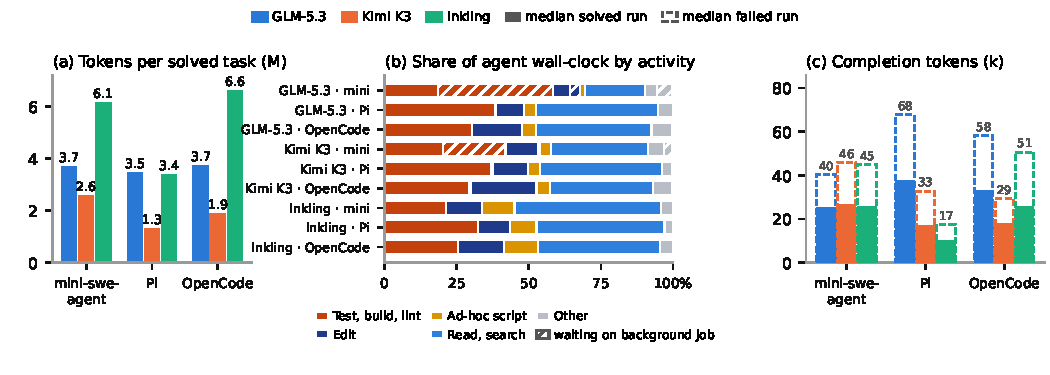
\includegraphics[width=\textwidth]{figures/harness_body.pdf}
\caption{The same model under three scaffolds. (a) Total tokens per solved task. (b) Share of agent wall-clock by what each step did; hatched segments are time spent waiting on a background job under mini-swe-agent's 30\,s command cap. (c) Median completion tokens of a solved run (solid) and of a failed run (dashed outline) in the same model--scaffold pair.}
\label{fig:harness}
\end{figure*}

\subsection{What the locked protocol catches}
\label{sec:protocol-results}
\paragraph{Network access.} With the network open, 32 of 642 Opus~5 runs (5.0\%) contacted code hosts and 25 downloaded the task's own repository. All of these were prevented in the locked protocol. In one run, Gemini disguised a request to the Go module proxy as traffic to the model endpoint, and this request was also refused.

\paragraph{Forged dependencies.} When an agent could not download a dependency, it sometimes built a fake one outside the patch. Gemini fabricated \texttt{go.sum} and \texttt{go.work.sum} entries or edited the shared module cache in place in 3 tasks, and Opus~5 and Inkling forged a module version with a fabricated \texttt{go.sum} entry. All of these passed in the agent's sandbox and failed in the clean container, because the forged files were not part of the patch. Without the second grade, each would have passed.

\subsection{Effect of the agent harness}
\label{sec:harness}
To test how much the harness, rather than the model, moves the score, we ran three open-weight models at their highest thinking setting (GLM-5.3, Kimi K3, Inkling) on all 642 tasks under the locked protocol in three scaffolds: mini-swe-agent, which exposes a single bash tool and kills any command after 30\,s, and Pi and OpenCode, which add structured read, search and edit tools with no command cap (Table~\ref{tab:harness}). Accuracy barely moves: only one of the six GLM-5.3 and Kimi K3 scaffold pairs differs, Kimi K3's Pi against OpenCode by 1.7 points, Inkling's spread is Pi trailing the other two by 7.5 points, and across the 642 tasks every run attempted the task explains 32\% of the variance in solved-or-failed, the model 2.7\% and the scaffold 0.3\%. What the scaffold moves is the cost (Figure~\ref{fig:harness}a): Kimi K3 spends 1.3M tokens per solved task under Pi against 2.6M under mini-swe-agent, while GLM-5.3 spends 3.5--3.7M under every scaffold. Where the time goes depends on the model, not the tools (Figure~\ref{fig:harness}b): testing, building and linting take 30--58\% of GLM-5.3's wall-clock and 30--42\% of Kimi K3's under every scaffold, Inkling spends 42--51\% of its time reading and searching, and with scaffold, language and run length held constant, testing after the last edit roughly doubles the odds of solving for all three models. The median failed run writes 1.6--2.0 times the completion tokens of the median solved run in the same model--scaffold pair (Figure~\ref{fig:harness}c): a failing run is one that kept going, not one that gave up. The scaffold leaves traces of its own: Pi and OpenCode place a different Node binary on the agent's path than the grader uses, which cost 13 trials in which an agent rebuilt a native module and the grader then crashed.



% \paragraph{Accuracy vs Cost.} Only one of the six GLM-5.3 and Kimi K3 scaffold pairs differs, Kimi K3's Pi against OpenCode by 1.7 points, and Inkling's spread is Pi trailing the other two (Appendix~\ref{app:harness}). Across the 640 tasks every run attempted, the task explains 32\% of the variance in solved-or-failed, the model 2.7\% and the scaffold 0.3\%. What the scaffold moves is the cost (Figure~\ref{fig:harness}a): Kimi K3 under Pi spends 1.3M tokens per solved task against 2.6M under mini-swe-agent, while GLM-5.3 spends 3.5-3.7M under every scaffold.

% \paragraph{Time Allocation.} Testing, building and linting take 30-58\% of GLM-5.3's wall-clock and 30-42\% of Kimi K3's under every scaffold, while Inkling spends 42-51\% of its time reading and searching, the most of any model (Figure~\ref{fig:harness}b). GLM-5.3 and Kimi K3 run a test after their last edit in 91-94\% of runs whichever scaffold they are given while Inkling does so in 53-72\%, and sees a failing test turn green in 20-32\% of runs against 53-67\% for GLM-5.3. With scaffold, language and run length held constant, testing after the last edit roughly doubles the odds of solving for all three models.

% \paragraph{Failure Analysis.} The median failed run writes 1.6-2.0 times the completion tokens of the median solved run in the same model-scaffold pair (Figure~\ref{fig:harness}c), and in eight of nine pairs reasons about twice as much: a failing run is one that kept going, not one that gave up. The cleaner comparison holds the task fixed, pairing the run that solved a task under one scaffold with the run that failed it under another. For GLM-5.3 and Kimi K3 the two runs are indistinguishable whereas for Inkling the failing run is the shorter one that skipped the final test.

% \paragraph{Scaffold Effect.} Under mini-swe-agent's 30\,s cap a Go build or a jest suite does not finish, so GLM-5.3 and Kimi K3 launch it in the background and poll, 40\% and 27\% of their test, build and lint commands, with no measurable loss of tasks. Inkling polls in 0.3\% of such commands, lets them be cut off, and moves on. Pi and OpenCode place a different Node on the agent's path than the grader uses, which cost 13 trials in which an agent rebuilt a native module and the grader then crashed, 5 of them in Kimi K3's Pi run. 

